\documentclass[a4paper,11pt, onecolumn]{article}

\usepackage[english]{babel}
\usepackage{amsmath, amssymb, graphicx, url, subfig, hyperref}

\newcommand{\cor}[1]{\textit{#1}} %corsivo
\newcommand{\gr}[1]{\textbf{#1}} %grassetto

\begin{document}

\title{9-month Research Report}
\author{
Marco Agnese \\
PhD student in Applied Mathematics \\
AMMP Section, Department of Mathematics, Imperial College London \\
London SW7 2AZ, UK \\
\url{m.agnese13@imperial.ac.uk}
}
\date{}
\maketitle

\section{Research topic}

\subsection{Two-phase Navier--Stokes problem}

My Ph.D. research project consists in the analytical study and numerical
implementation of a finite element method to solve a mathematical model of
two-phases Navier--Stokes flow in 2-D and 3-D. Numerical methods for these flows
have many important applications, which range from fuel injection in engines to
biomedical engineering. Two-phase flow is a free boundary problem since the
evolution of the interface is not prescribed but it is an unknown of the
problem.
\newline

In the literature there are different computational techniques to deal
with the numerical treatment of the unknown interface. One class of approaches
is based on interface capturing methods using an indicator function to describe
the interface. The \cor{volume of fluid method} and the \cor{level set method}
fall into this category. In the former, the characteristic function of one of
the phases is approximated numerically, see e.g.
\cite{HirtN81,RenardyR02,Popinet09}; whereas in the latter, the interface is
given as the level set of a function, which has to be determined, see e.g.
\cite{GrossR07}.

In \cor{phase field methods} the interface is assumed to have a small,
but positive, thickness and an additional parabolic equation, defined in the
whole domain, has to be solved in these so-called diffuse interface models, see
e.g. \cite{HohenbergH77,AndersonMW98,LowengrubT98,Feng06,KaySW08,AbelsGG12} for
details.

Lastly, in \cor{front tracking methods} the interface is approximated
by a polyhedral surface, \cite{DeckelnickDE05}, and equations on the surface
mesh have to be coupled to quantities defined on the bulk mesh, see e.g.
\cite{UnverdiT92,Bansch01,Tryggvason_etal01,GanesanMT07}.
\newline

Recently in \cite{spurious,fluidfbp} a novel front-tracking method was
developed which has good mesh properties. We note that in
\cite{spurious,fluidfbp} an \cor{unfitted approach} was considered, which means
that the numerical approximation of the interface is totally independent of the
bulk mesh. The aim of my research project is to extend the ideas from
\cite{spurious,fluidfbp} to the \cor{fitted approach}, where the discrete
interface approximation is given as an union of edges/faces of the bulk mesh
elements.
\newline

We consider two-phase flows in a given domain
$\Omega\subset\mathbb{R}^d$, where $d=2$ or $d=3$. The domain $\Omega$ contains
two different immiscible incompressible phases (liquid-liquid or liquid-gas)
which for all $t\in[0,T]$ occupy time dependent regions $\Omega_+(t)$ and
$\Omega_-(t):=\Omega\setminus\overline{\Omega}_+(t)$ and which are separated by
an interface $(\Gamma(t))_{t\in[0,T]}$, $\Gamma(t)\subset\Omega$.

Moreover we assume that $(\Gamma(t))_{t\in [0,T]}$ is a sufficiently
smooth evolving hypersurface.
\newline

Let $\rho(t) = \rho_+\,\mathbf{1}_{\Omega_+(t)} +
\rho_-\,\mathbf{1}_{\Omega_-(t)}$, with $\rho_\pm \in \mathbb{R}_{\geq0}$,
denote the fluid densities, where here and throughout $\mathbf{1}_{\mathcal{A}}$
defines the characteristic function for a set $\mathcal{A}$. Denoting by $\vec u
: \Omega \times [0, T] \to \mathbb{R}^d$ the fluid velocity, by
$\underline{\underline{\sigma}} : \Omega \times [0,T] \to \mathbb{R}^{d \times
d}$ the stress tensor, and by $\vec f : \Omega \times [0, T] \to \mathbb{R}^d$ a
possible forcing, the incompressible Navier--Stokes equations in the two phases
are given by
\begin{subequations}
 \begin{alignat}{2}
  \rho\,(\vec u_t + \vec u \,\cdot\,\nabla\,\vec u)
  - \nabla\,\cdot\,\underline{\underline{\sigma}} & = \vec f := \rho\,\vec f_1
  + \vec f_2 \qquad &&\mbox{in }
  \Omega_\pm(t)\,, \label{eq:NSa} \\
  \nabla\,\cdot\,\vec u & = 0 \qquad &&\mbox{in } \Omega_\pm(t)\,,
  \label{eq:NSb} \\
  \vec u & = \vec 0 \qquad &&\mbox{on } \partial_1\Omega\,, \label{eq:NSc} \\
  \vec u \,\cdot\,\vec{n} = 0\,,\quad
  [\underline{\underline{\sigma}}\,\vec{n} + \beta\,\vec u]\,\cdot\,\vec{t}& = 0
  \quad\forall\ \vec{t} \in \{\vec{n}\}^\perp
  \qquad &&\mbox{on } \partial_2\Omega\,,
  \label{eq:NSd}
 \end{alignat}
\end{subequations}
where $\partial\Omega =\partial_1\Omega \cup \partial_2\Omega$, with
$\partial_1\Omega \cap \partial_2\Omega =\emptyset$, denotes the boundary of
$\Omega$ with outer unit normal $\vec{n}$ and $\{\vec{n}\}^\perp := \{ \vec{t}
\in \mathbb{R}^d : \vec{t} \,\cdot\,\vec{n} = 0\}$. Hence (\ref{eq:NSc})
prescribes a no-slip condition on $\partial_1\Omega$, while (\ref{eq:NSd})
prescribes a general slip condition on $\partial_2\Omega$. Here we assume that
$\beta \geq 0$ and note that $\beta = 0$ corresponds to the so-called free-slip
conditions.

Moreover, the stress tensor in (\ref{eq:NSa}) is defined by
\begin{equation} \label{eq:sigma}
 \underline{\underline{\sigma}} = \mu \,(\nabla\,\vec u + (\nabla\,\vec u)^T) -
 p\,\underline{\underline{Id}}\,,
\end{equation}
where $\underline{\underline{Id}} \in \mathbb{R}^{d \times d}$ denotes the
identity matrix, $p : \Omega \times [0, T] \to \mathbb{R}$ is the pressure and
$\mu(t) = \mu_+\,\mathbf{1}_{\Omega_+(t)} + \mu_-\,\mathbf{1}_{\Omega_-(t)}$,
with $\mu_\pm \in \mathbb{R}_{>0}$, denotes the dynamic viscosities in the two
phases.
\newline

On the free surface $\Gamma(t)$, the following conditions need to hold:
\begin{subequations}
 \begin{alignat}{2}
  [\vec u]_-^+ & = \vec 0 \qquad &&\mbox{on } \Gamma(t)\,, \label{eq:1a} \\
  [\underline{\underline{\sigma}}\,\vec \nu]_-^+ & = -\gamma\,\varkappa\,\vec
  \nu \qquad &&\mbox{on } \Gamma(t)\,, \label{eq:1b} \\
  \mathcal{V} &= \vec u\,\cdot\,\vec \nu \qquad &&\mbox{on } \Gamma(t)\,,
  \label{eq:1c}
 \end{alignat}
\end{subequations}
where $\gamma>0$ is the surface tension coefficient where we have adopted the
sign convention that $\varkappa$ is negative where $\Omega_-(t)$ is locally
convex. Moreover, $\vec{\nu}$ is the unit normal to the interface and
\eqref{eq:1c} is a geometric PDE, see Sec.\ref{subsec:math_form_interface} for
more details. As usual, $[\vec u]_-^+ := \vec u_+ - \vec u_-$ and
$[\underline{\underline{\sigma}}\,\vec\nu]_-^+ :=
\underline{\underline{\sigma}}_+\,\vec\nu -
\underline{\underline{\sigma}}_-\,\vec\nu$ denote the jumps in velocity and
normal stress across the interface $\Gamma(t)$.
\newline

The system (\ref{eq:NSa}--d), (\ref{eq:sigma}), (\ref{eq:1a}--c) is
closed with the initial conditions
\begin{equation} \label{eq:1d}
 \Gamma(0) = \Gamma_0 \,, \qquad \rho(\cdot,0)\,\vec u(\cdot,0) =
\rho(\cdot,0)\,\vec u_0 \qquad \mbox{in } \Omega\,,
\end{equation}
where $\Gamma_0 \subset \Omega$ and $\vec u_0 : \Omega \to \mathbb{R}^d$ are
given initial data.
\newline

My project goal is to extend \cite{spurious,fluidfbp} to the fitted
case which will require combining \cite{spurious,fluidfbp} with ideas from the
\cor{ALE} approach, see e.g. \cite{HughesLZ81,Ganesan06,GerbeauLL06}.

\subsection{Mathematical description of the interface}
\label{subsec:math_form_interface}

As starting point, I consider the simple problem of purely geometric PDEs.
Several different methods to approximate evolving surfaces can be found in the
literature, these methods can be divided in explicit and implicit, see e.g.
\cite{DeckelnickDE05}. The parametric approach is an example of an explicit
method which involves seeking a parametrization over a base surface (e.g. a
sphere). On the other hand, the surface can be represented as the zero level set
of a certain function giving rise to the implicit method known as level set
method. Another implicit method is the so called phase field method which
approximates the interface by a zero level set of a phase field satisfying a PDE
depending on a new parameter.
\newline

We choose to use a parametric approach which consists of a description
of the hypersurface $\Gamma(t)$ as
\begin{equation}\label{eq:parametric_hypersurface}
 \Gamma(t)=\vec{x}(\cdot,t)(M)
\end{equation}
where $M\subset\mathbb{R}^{d}$ is the reference manifold and
\begin{equation}\label{eq:position_vector}
 \vec{x}:M\times[0,T)\rightarrow\mathbb{R}^{d}
\end{equation}
is one unknown of the problem. Finally $\vec{x}(\vec{p},t)$, $\vec{p}\in M$, is
the position vector at a certain time $t$ and at a certain point $\vec{p}$ of
the reference manifold. All the geometrical quantities of the hypersurface (e.g.
curvature) can be expressed as derivatives of the parametrization.
\newline

An equation which describes the motion of a surface prescribing the normal
velocity is called \cor{geometric PDE}. More precisely a general geometric
evolution equation has the following form
\begin{equation}\label{eq:geometric_pde}
 V=f(\vec{x},\vec{\nu},\varkappa),\qquad\mbox{on }\Gamma(t),
\end{equation}
where $\vec{\nu}$ is the normal direction and $\varkappa$ is the sum of the
principal curvatures of $\Gamma(t)$. One of the simplest geometric PDEs is the
one which arises from motion by \cor{mean curvature}, see e.g.
\cite{DeckelnickDE05},
\begin{equation}\label{eq:mean_curvature}
 V=-\varkappa,\qquad\mbox{on }\Gamma(t).
\end{equation}

This equation describes a surface evolving in such a way that its own normal
velocity is equal to the sum of the $d-1$ principal curvatures of $\Gamma(t)$.
\newline

Another important geometric PDE is the one which arises from motion by
\cor{surface diffusion}
\begin{equation}\label{eq:surface_diff}
 V=-\Delta_{\Gamma(t)} \varkappa,\qquad\mbox{on }\Gamma(t)
\end{equation}
where $\Delta_{\Gamma(t)}$ is the \cor{Laplace--Beltrami} operator, also called
surface Laplacian, defined as
\begin{equation}\label{eq:laplace_beltrami}
 \Delta_{\Gamma(t)}f(\vec{p}) =
 \nabla_{\Gamma(t)}\cdot\nabla_{\Gamma(t)}f(\vec{p} ) ,\qquad
 \vec{p}\in\Gamma(t).
\end{equation}
Here $\nabla_{\Gamma(t)}$ is the \cor{tangential gradient} defined as
\begin{equation}\label{eq:tangent_gradient}
 \nabla_{\Gamma(t)}f(\vec{p})=\nabla f(\vec{p})-\nabla
 f(x)\cdot\vec{\nu}(\vec{p})\vec{\nu}(\vec{p}),\qquad \vec{p}\in\Gamma(t).
\end{equation}

It can be shown that both \eqref{eq:mean_curvature} and
\eqref{eq:surface_diff} decrease the surface area of $\Gamma(t)$ over time.
Moreover \eqref{eq:surface_diff} conserves the volume enclosed by $\Gamma(t)$,
which means that a sphere remains exactly the same sphere when it evolves
according to surface diffusion. See \cite{DeckelnickDE05} for more details on
geometric evolution equations and their numerical approximation.

\subsection{Finite element formulation of the interface}

The \cor{Finite Element Method} which I use is based on the seminal paper
\cite{Dziuk91} and I refer to the ones described in
\cite{triplej,triplejMC,gflows3d}. The surface diffusion problem
\eqref{eq:surface_diff} can be rewritten as a system of second order equations
\begin{equation}\label{eq:surf_diff_sys}
 \begin{cases}
  \vec{x}_t\cdot\vec{\nu}=-\Delta_{\Gamma(t)} \varkappa,\\
  \varkappa\vec{\nu}=\Delta_{\Gamma(t)}\vec{x},
 \end{cases}
\end{equation}
where we have used the fact that the \cor{normal velocity} can be expressed as a
function of the parametrization
\begin{equation}
 V=\vec{x}_t\cdot\vec{\nu}.
\end{equation}
The second equation, instead, is a well-known identity from surface geometry.
\newline

The FEM scheme for \eqref{eq:surf_diff_sys} from \cite{gflows3d} assumes the
following formulation
\begin{equation}\label{eq:fem_surf_diff}
 \begin{cases}
  \langle \frac{\vec{X}^{m + 1} - \vec{X}^{m}}{\tau_m},
  \chi\vec{\nu}^m\rangle_{\Gamma^m}^{h} - \langle\nabla_{
  \Gamma^m}\kappa^{m+1}, \nabla_{\Gamma^m}\chi \rangle_{\Gamma^m}^{h} = 0,\\
  \langle\kappa^{m+1}\vec{\nu}^m,
  \vec{\eta}\rangle_{\Gamma^m}^{h} + \langle\nabla_{\Gamma^m}\vec{X}^{m + 1},
  \nabla_{\Gamma^m}\vec{\eta} \rangle_{\Gamma^m}=0
 \end{cases}
\end{equation}
$\forall\vec{\eta}\in\underline{V}(\Gamma^m)$ and $\forall\chi\in W(\Gamma^m)$.
These spaces of test functions are defined as
\begin{equation}\label{eq:space_test_functions}
 \underline{V}(\Gamma^m) := \{\vec{\chi}\in C(\Gamma^m,\mathbb{R}^d) :
\vec{\chi}|_{\sigma_j^m}\textrm{ is linear }\forall j=1\rightarrow J\} :=
[W(\Gamma^m)]^d\subset H^1(\Gamma^m,\mathbb{R}^d)
\end{equation}
where $W(\Gamma^m)\subset H^1(\Gamma^m)$ is the space of scalar continuous
piecewise linear functions on $\Gamma^m$. Here $\Gamma^m$ is the polyhedral
surface which approximates the surface $\Gamma (t^m)$ at time $t^m$ and
$\{\sigma_j^m\}_{j=1}^J$ is a family of mutually disjoint open triangles such
that $\Gamma^m=\cup_{j=1}^J\overline{\sigma_j^m}$.
\newline

Moreover $\langle\cdot,\cdot\rangle_{\Gamma^m}$ is the $L^2$ inner product over
the current polyhedral surface
\begin{equation}\label{}
 \langle u,v\rangle_{\Gamma^m} = \int_{\Gamma^m}uv\,\mathrm{d}s,\qquad\forall
  u,v\in L^2(\Gamma^m),
\end{equation}
and similarly for $\vec{u},\vec{v}\in L^2(\Gamma^m,\mathbb{R}^d)$. In addition,
$\langle \cdot,\cdot\rangle_{\Gamma^m}^h$ is a mass lumped inner product with
the vertices of each triangle of the mesh as quadrature points.
\newline

For what concerns the mean curvature flow, the system of second order equations
is
\begin{equation}\label{eq:mean_curvature_sys}
 \begin{cases}
  \vec{x}_t\cdot\vec{\nu}=-\varkappa,\\
  \varkappa\vec{\nu}=\Delta_{\Gamma(t)}\vec{x},
 \end{cases}
\end{equation}
and the FEM formulation from \cite{gflows3d} is
\begin{equation}\label{eq:fem_mean_curvature}
 \begin{cases}
  \langle \frac{\vec{X}^{m + 1} - \vec{X}^{m}}{\tau_m},
  \chi\vec{\nu}^m\rangle_{\Gamma^m}^{h} - \langle\kappa^{m+1}, \chi
  \rangle_{\Gamma^m}^{h}=0,\\
  \langle\kappa^{m+1}\vec{\nu}^m, \vec{\eta}\rangle_{\Gamma^m}^{h} +
  \langle\nabla_{\Gamma^m}\vec{X}^{m + 1}, \nabla_{\Gamma^m}\vec{\eta}
  \rangle_{\Gamma^m}=0.
 \end{cases}
\end{equation}

\subsection{Algebraic formulation of the interface}

As regards the mean curvature flow, \eqref{eq:fem_mean_curvature}, the
corresponding algebraic system of equations can be written as

\begin{equation}\label{eq:algebraic_mean_curvature}
 \begin{pmatrix}
  \tau_m \, M_m & - \, \vec{N}_{m}^{T} \\
  \vec{N}_m & \vec{A}_m
 \end{pmatrix}
 \begin{pmatrix}
  \kappa^{m + 1} \\
  \delta \vec{X}^{m + 1}
 \end{pmatrix}
 =
 \begin{pmatrix}
  0 \\
  - \vec{A}_m \, \vec{X}^{m}
 \end{pmatrix} ,
\end{equation}
while, for the system of equations describing the surface diffusion,
\eqref{eq:fem_surf_diff}, the algebraic system is
\begin{equation}\label{eq:algebraic_surf_diff}
 \begin{pmatrix}
  \tau_m \, A_m & - \, \vec{N}_{m}^{T} \\
  \vec{N}_m & \vec{A}_m
 \end{pmatrix}
 \begin{pmatrix}
  \kappa^{m + 1} \\
  \delta \vec{X}^{m + 1}
 \end{pmatrix}
 =
 \begin{pmatrix}
  0 \\
  - \vec{A}_m \, \vec{X}^{m}
 \end{pmatrix}.
\end{equation}
We can notice that the only difference between the above systems occurs in the
upper-left entry of the matrix.
\newline

The entries of the matrix are defined as
\begin{eqnarray}\label{eq:algebraic_entries}
 \left[ M_m \right]_{kl} & := & \langle \phi_k^m \, , \phi_l^m \rangle_m^h, \\
 \left[ \vec{N}_m \right]_{kl} & := & \int_{\Gamma^m} \pi^h \left[ \phi_k^m ,
 \phi_l^m \right] \vec{\nu}^m \mathrm{d}s, \\
 \left[ A_m \right]_{kl} & := & \langle \nabla_s \phi_k^m \, , \nabla_s
 \phi_l^m \rangle_m,
\end{eqnarray}
where $\{\phi_k\}$ are the basis functions of the finite element space of
piecewise linear continuous functions $W(\Gamma^m)$ and
\begin{equation}\label{eq:algebraic_entries_vector}
 [\vec{A}_m]_{kl} := [A_m]_{kl} \vec{Id},
\end{equation}
where $\vec{Id}$ is the identity matrix.
\newline

The linear systems \eqref{eq:algebraic_mean_curvature} and
\eqref{eq:algebraic_surf_diff} are invertible under a suitable assumption on the
triangulation at each time step, see \cite{gflows3d}. Hence they can be solved
with a sparse factorization package such as \verb|UMFPACK|, see \cite{Davis04}.
\newline

Alternately, the algebraic system \eqref{eq:algebraic_mean_curvature} can be
solved with a \cor{Schur complement} approach:
\begin{subequations}
 \begin{eqnarray}
  \kappa^{m + 1} & = & \frac{1}{\tau_m} M_m^{-1} \vec{N}^{T}_m \, \delta
  \vec{X}^{m + 1} \label{subeq:schur_mcf_1} , \\
  (\vec{A}_m + \frac{1}{\tau_m} \vec{N}_m M_m^{-1} \vec{N}^{T}_m) \, \delta
  \vec{X}^{m + 1} & = & - \vec{A}_m \, \vec{X}^{m} , \label{subeq:schur_mcf_2}
 \end{eqnarray}
\end{subequations}
where \eqref{subeq:schur_mcf_2} is symmetric and positive definite.

\subsection{Software used}

In order to simulate numerically the evolution governed by mean curvature flow
and surface diffusion I have chosen to use the \verb|DUNE| framework (acronym
for \verb|Distributed| \verb|and| \verb|Unified| \verb|Numerics|
\verb|Environment|)), see
\cite{dunegridpaperI08,dunegridpaperII08,ISTL,ISTLParallel}.

\verb|DUNE| is a modular toolbox for solving partial differential equations
with grid-based methods. It implements slim interfaces allowing an efficient use
of legacy and new libraries. Moreover it is coded with modern \verb|C++|
programming techniques levering heavily on template meta-programming. These
techniques enable very different implementations of the same concept (like
grids, solvers) using a common interface at a very low overhead. For this
reasons, this framework ensures efficiency in scientific computations and
supports high-performance computing applications.

\verb|DUNE| is based on the following main principles:
\begin{itemize}
 \item separation of data structures and algorithms by abstract interfaces;
 \item efficient implementation of these interfaces using generic programming
 techniques;
 \item reuse of existing finite element packages with a large body of
 functionality.
\end{itemize}

For what concern the FEM discretisation, I use the module \verb|dune-fem|,
based on the \verb|dune-grid| interface library, see \cite{dunefempaper10}.
This module aims at extending \verb|dune-grid| by a number of discretisation
algorithms for the resolution of non-linear systems of partial differential
equations.

The main concept is that of a \cor{spatial discrete operator} which models a
mapping between two discrete function spaces: $L_h : U_h \to V_h$. Basic
operators can be combined to construct more complex operators.

Finally, \verb|dune-fem| offers different solvers, both direct and iterative;
unfortunately the direct solvers are only sequential up to now.
\newline

In order to construct the discrete operators, the user has to choose a
continuous function space, a set of basis functions over it and a view of the
underlying grid. The view determines the part of the grid on which the functions
are defined. So far, it is possible to use discontinuous and Lagrange finite
element spaces.

\subsection{Preliminary numerical results}

I implemented a \verb|DUNE| module, called \verb|dune-interface|, to simulate
surface diffusion, \eqref{eq:fem_surf_diff}, and  mean curvature flow,
\eqref{eq:fem_mean_curvature}.

This module can simulate surfaces embedded both in 2-D and in 3-D. Moreover, it
supports \verb|ALBERTA|, see \cite{Alberta}, and \verb|ALUGrid|, see
\cite{alugrid}, as grid managers. More precisely, \verb|ALUGrid| manages only
2-D surfaces but it can be used both sequentially and in parallel (using
\verb|MPI|). On the other hand, \verb|ALBERTA| supports 1-D and 2-D surfaces but
it can be run only sequentially.
\newline

When running the code sequential, the module uses the \verb|UMFPACK| direct
solver. Finally, the initial mesh is created using \verb|GMSH|, see
\cite{GeuzaineR09}, and it is read by the module from a \verb|.msh| file.
\newline

To test my module, I performed some simulations reported in the following
section.

\subsubsection{Mean curvature flow with a sphere as initial condition}

As regards the mean curvature flow, the simplest case is to use a sphere as the
initial condition, see \cite{Ilmanen98}. Indeed, the sphere shrinks without
changing shape since the curvature is the same all around. In this case
\eqref{eq:mean_curvature} can be rewritten as
\begin{equation}\label{eq:mcf_sphere}
 \frac{\mathrm{d}R}{\mathrm{d}t}=-\frac{d-1}{R},\qquad R(0)=R_0
\end{equation}
where $R(t)$ is the radius of the sphere and $d$ is the dimension of the world
where the sphere is embedded. Equation \eqref{eq:mcf_sphere} has the following
analytical solution
\begin{equation}\label{eq:mcf_sphere_solution}
 R(t)=\sqrt{R_0^2-2(d-1)t},
\end{equation}
so the sphere disappears at time
\begin{equation}\label{eq:extinction_time}
 t_{e}=\frac{R_0^2}{2(d-1)}.
\end{equation}

\begin{figure}[htbp]
 \centering
 \subfloat[][]{
 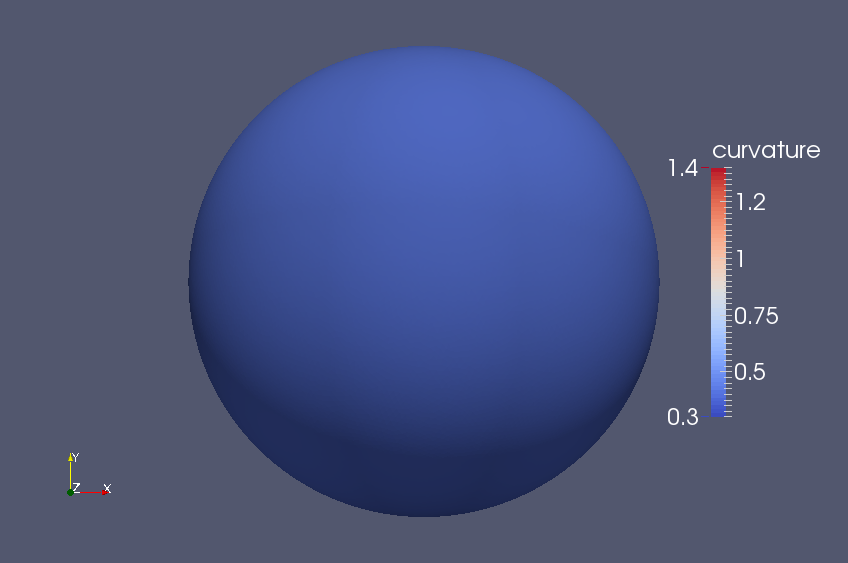
\includegraphics[width=.45\textwidth]{figures/mc_sphere_01_00.png}}\quad
 \subfloat[][]{
 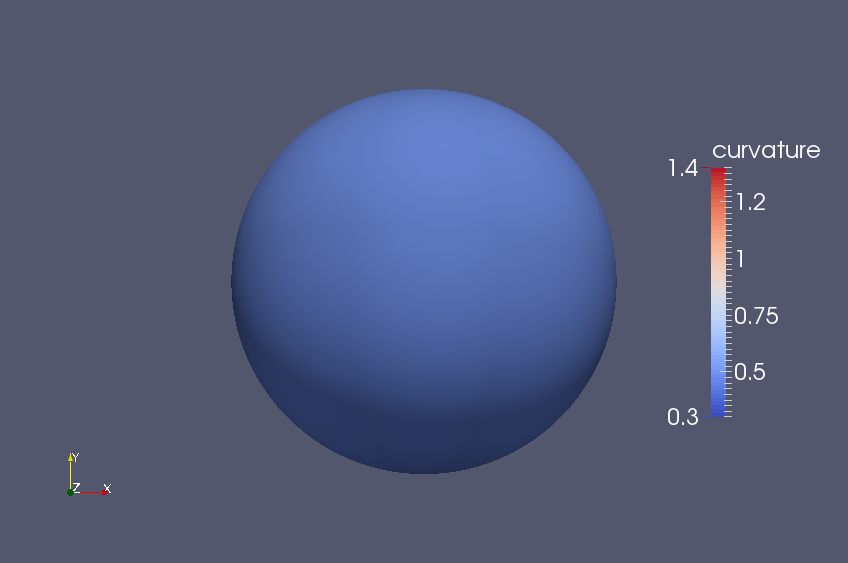
\includegraphics[width=.45\textwidth]{figures/mc_sphere_01_20.png}}\\
 \subfloat[][]{
 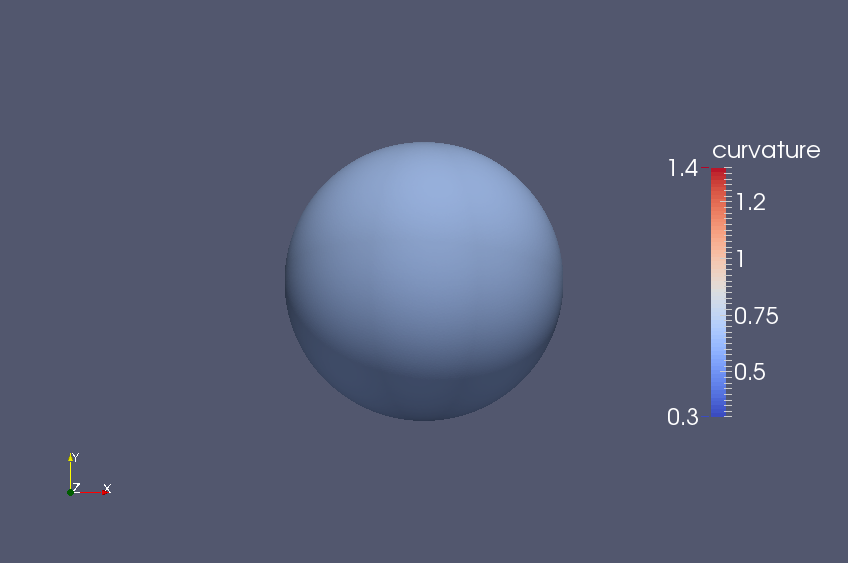
\includegraphics[width=.45\textwidth]{figures/mc_sphere_01_40.png}}\quad
 \subfloat[][]{
 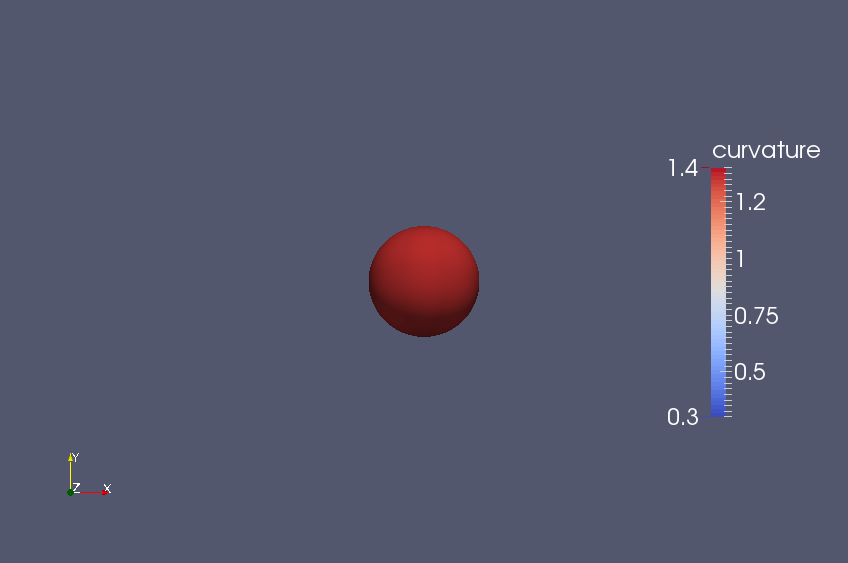
\includegraphics[width=.45\textwidth]{figures/mc_sphere_01_60.png}}
 \caption{Mean curvature flow with a sphere as initial condition.}
 \label{fig:mcf_sphere}
\end{figure}

In Fig.\ref{fig:mcf_sphere} there are 4 snapshots of the simulation at time
$t=0.1$, $t=2.1$, $t=4.1$ and $t=6.1$ respectively. The initial sphere has
radius $R_0=5$; obviously $d=3$ since the simulation is 3-D. In this case, the
extinction time, \eqref{eq:extinction_time}, is $t_e=\frac{25}{4}=6.25$. The
number of mesh elements is 74770 and there are 37387 nodes. The time step is
constant and equal to $\tau=0.1$.
\newline

We can see that the evolution is consistent to what was expected.

\subsubsection{Mean curvature flow with a cube as initial condition}

Since mean curvature flow \eqref{eq:mean_curvature} is a parabolic equation it
will have a short-term smoothing effect on the surface. However, the surface can
become singular later. It has been proven, \cite{Huisken84}, that if $\Gamma(0)$
is a bounded convex surface, than $\Gamma(t)$ becomes more and more nearly
spherical as it shrinks, and at the instant it vanishes, it is asymptotic to the
shrinking sphere given above.
\newline

\begin{figure}[htbp]
 \centering
 \subfloat[][]{
 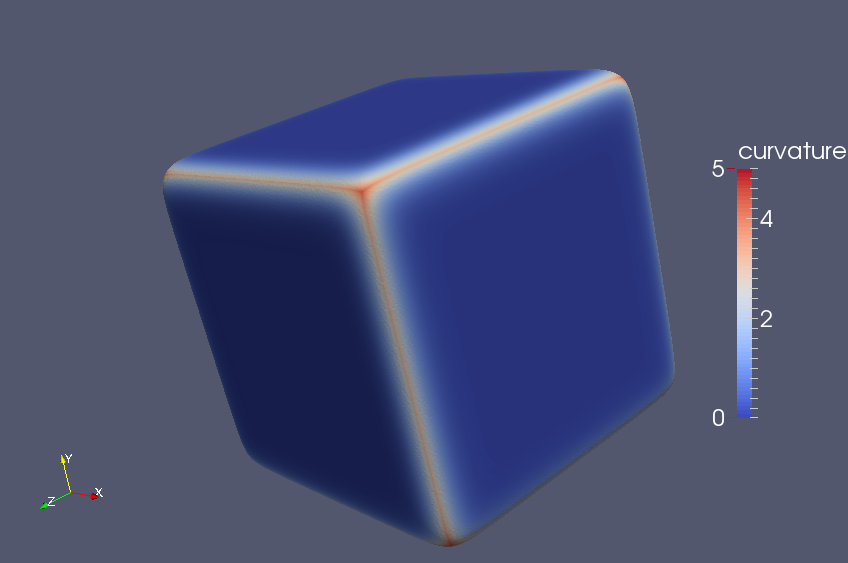
\includegraphics[width=.45\textwidth]{figures/mc_cube_01_00.png}}\quad
 \subfloat[][]{
 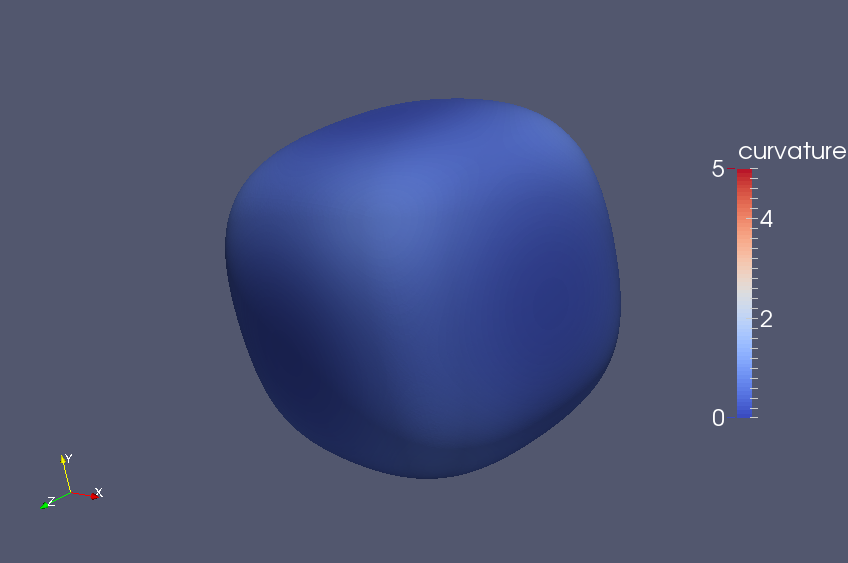
\includegraphics[width=.45\textwidth]{figures/mc_cube_01_20.png}}\\
 \subfloat[][]{
 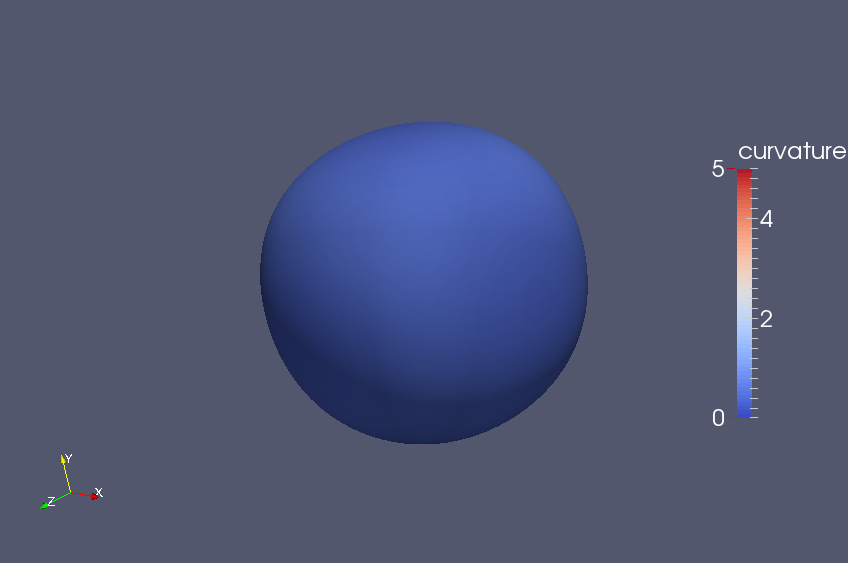
\includegraphics[width=.45\textwidth]{figures/mc_cube_01_40.png}}\quad
 \subfloat[][]{
 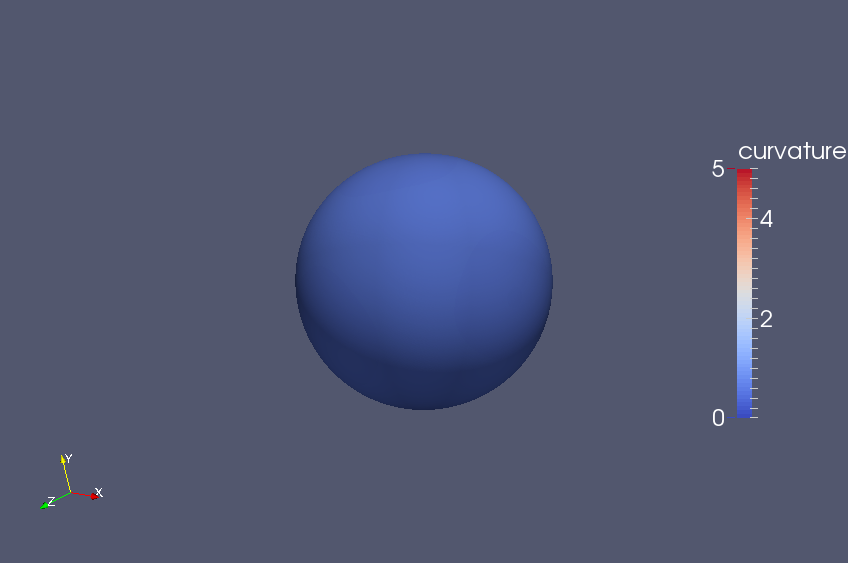
\includegraphics[width=.45\textwidth]{figures/mc_cube_01_60.png}}
 \caption{Mean curvature flow with a cube as initial condition.}
 \label{fig:mcf_cube}
\end{figure}

In Fig. \ref{fig:mcf_cube} there are 4 snapshots of the simulation at time
$t=0.1$, $t=2.1$, $t=4.1$ and $t=6.1$ respectively. The initial cube  has edges
of length $L=10$. The number of mesh elements is 158420 and there are 79212
nodes. The time step is constant and equal to $\tau=0.1$.
\newline

As expected, there is a smoothing effect and the cube shrinks becoming slowly a
sphere.

\subsubsection{Surface diffusion with an ellipsoid as initial condition}

In order to test the surface diffusion I have used as initial condition an
ellipsoid. The ellipsoid should evolve towards a sphere and then become
stationary. Moreover the enclosed volume should remain constant during all the
computation.

\begin{figure}[htbp]
 \centering
 \subfloat[][]{
 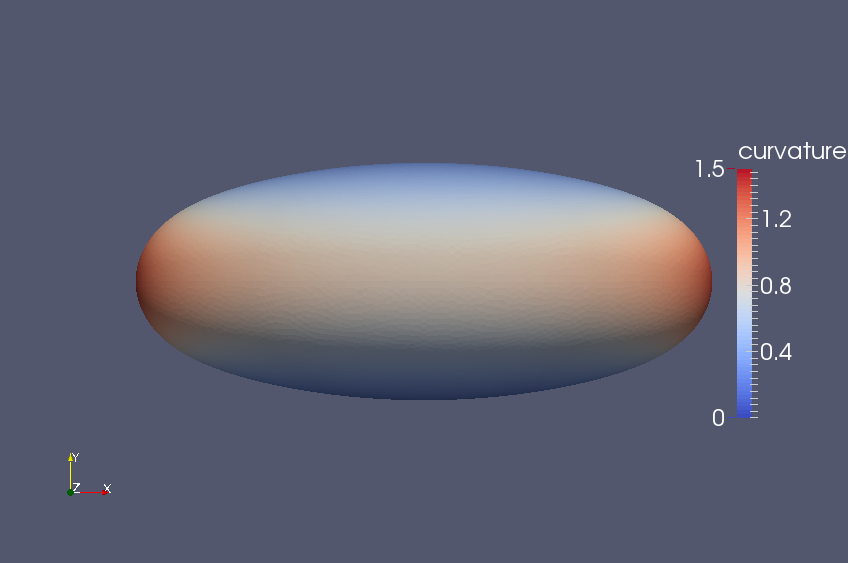
\includegraphics[width=.45\textwidth]{figures/sd_ellipsoid_01_00.png}}\quad
 \subfloat[][]{
 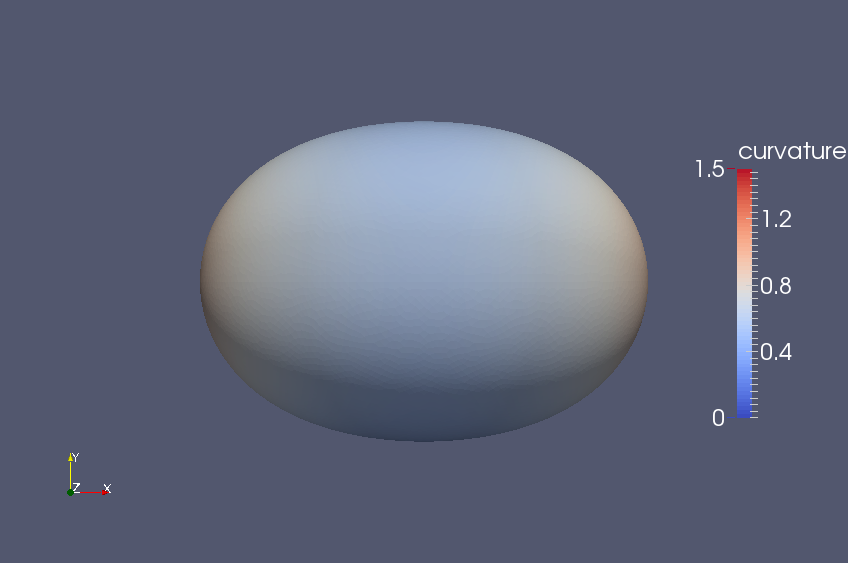
\includegraphics[width=.45\textwidth]{figures/sd_ellipsoid_01_50.png}}\\
 \subfloat[][]{
 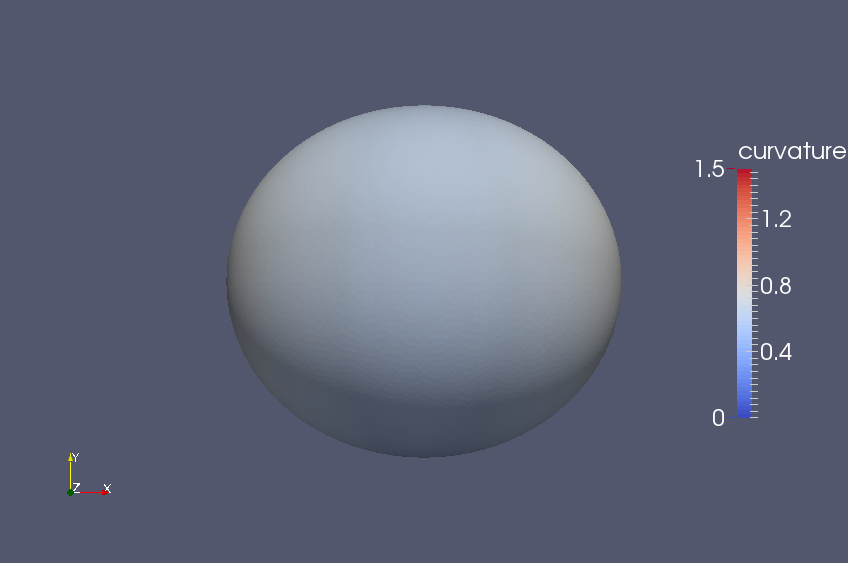
\includegraphics[width=.45\textwidth]{figures/sd_ellipsoid_01_100.png}}\quad
 \subfloat[][]{
 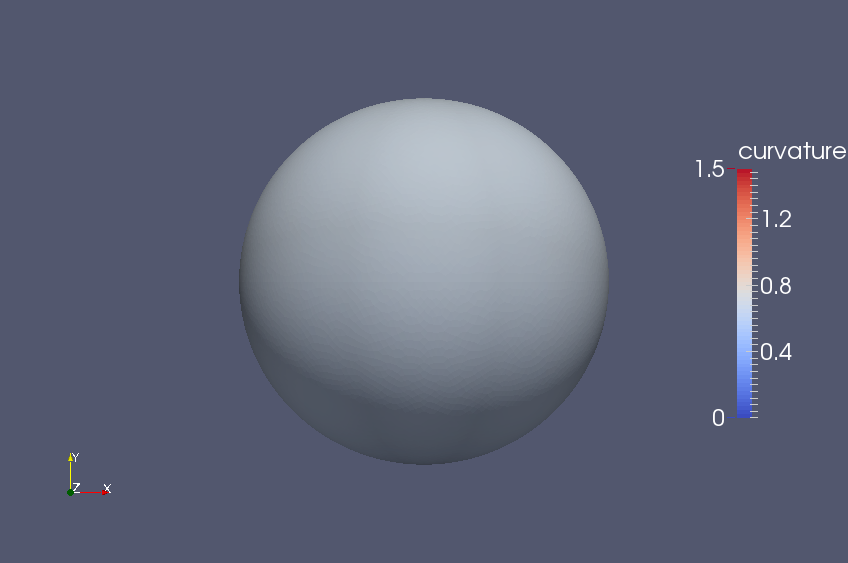
\includegraphics[width=.45\textwidth]{figures/sd_ellipsoid_01_200.png}}
 \caption{Surface diffusion with an ellipsoid as initial condition.}
 \label{fig:sd_ellipsoid}
\end{figure}

In Fig. \ref{fig:sd_ellipsoid} there are 4 snapshots of the simulation at time
$t=0.1$, $t=5.1$, $t=10.1$ and $t=20.1$ respectively. The initial ellipsoid has
semi-axes of length 5, 2 and 3 along the x-axis, y-axis and z-axis,
respectively. The number of mesh elements is 31464 and there are 15734 nodes.
The time step is constant and equal to $\tau=0.1$.
\newline

Also in this case the numerical result is consistent.

\subsubsection{Surface diffusion with an ellipse as initial condition}
\label{subsubsec:sd_ellipse}

Finally, in order to testing the case of a 1-D surface (curve), I have used as
initial condition an ellipse that then evolves accord to surface diffusion. Also
for the ellipse we expect an evolution towards a circle. Moreover the enclosed
area should remain constant during all the computation.

\begin{figure}[htbp]
 \centering
 \subfloat[][]{
 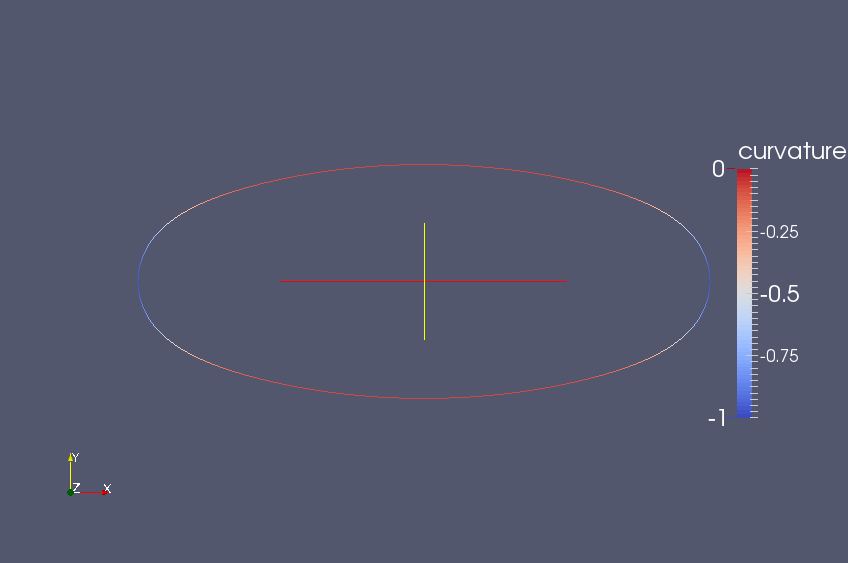
\includegraphics[width=.45\textwidth]{figures/sd_ellipse_01_00.png}}\quad
 \subfloat[][]{
 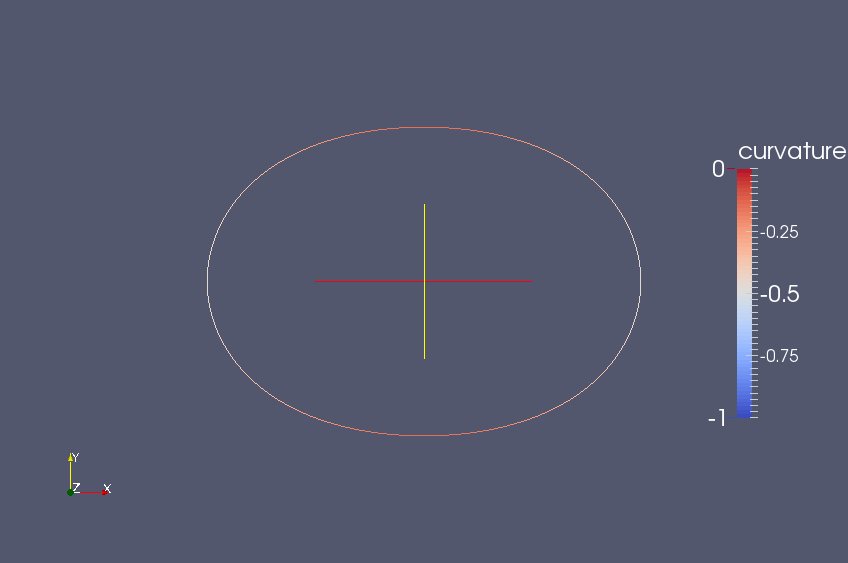
\includegraphics[width=.45\textwidth]{figures/sd_ellipse_01_100.png}}\\
 \subfloat[][]{
 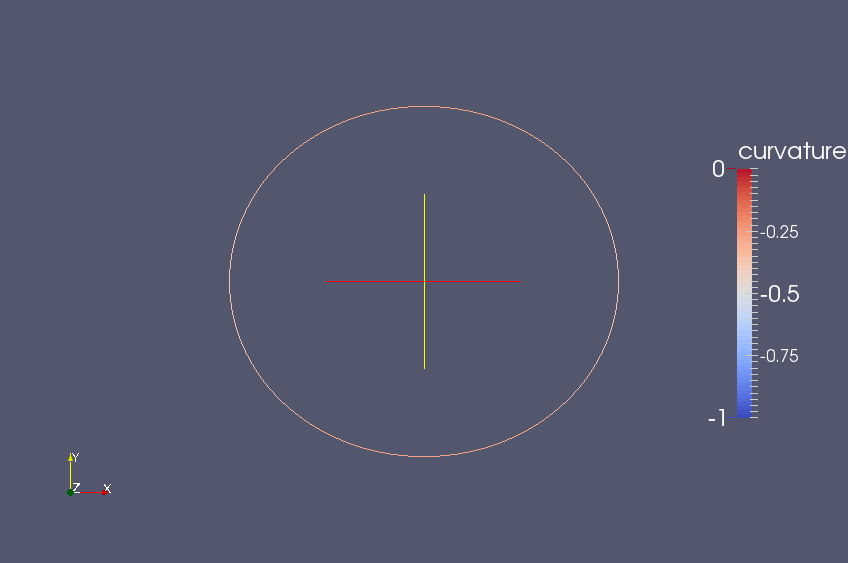
\includegraphics[width=.45\textwidth]{figures/sd_ellipse_01_200.png}}\quad
 \subfloat[][]{
 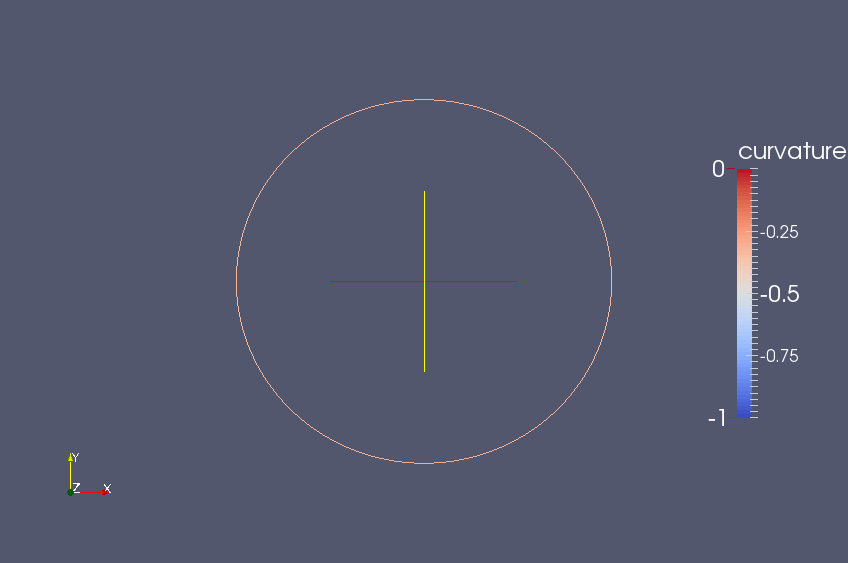
\includegraphics[width=.45\textwidth]{figures/sd_ellipse_01_299.png}}
 \caption{Surface diffusion with an ellipse as initial condition.}
 \label{fig:sd_ellipse}
\end{figure}

In Fig. \ref{fig:sd_ellipse} there are 4 snapshots of the simulation at time
$t=0.1$, $t=10.1$, $t=20.1$ and $t=30.0$ respectively. The initial ellipse has
semi-axes of length 5 and 3 along the x-axis and y-axis respectively. The number
of mesh elements is 232 and there are 232 nodes. The time step is constant and
equal to $\tau=0.1$.
\newline

As before, we have obtained what expected.

\subsection{Grid and sub--grid}

So far I have described how to solve the geometric PDE over the interface.
However, for the project, we also need to couple an equation for the bulk (e.g.
Navier--Stokes).

Unfortunately the core modules of \verb|DUNE| do not allow to have a grid with a
problem defined on it and a sub-grid, of lower dimension, with another problem.
To tackle this issue I wrote another module to manage these complex types of
grids called \verb|dune-dynamic-grid|.
\newline

This module offers different functionalities which are essential for my
project. The most important are:
\begin{itemize}
 \item dynamic grids;
 \item coupled grid--sub-grid;
 \item re-meshing.
\end{itemize}

In the following sections I will describe very briefly these features.

\subsubsection{Dynamic grids}

\verb|dune-grid| is the \verb|DUNE| core module which provides the interface for
every grid. All the grids, once created, cannot be modified.

The only operation which modifies the grid is the refinement, performed usually
by splitting one edge. When the user performs a refinement, a level in the
hierarchical grid is added for all the elements which are refined.
\newline

Since the problems which I am dealing with modify the grid at every time step, I
need an efficient way to change the values of the grid without recreating the
mesh at each time step (very inefficient).

\verb|dune-dynamic-grid| implements a new type of grid which maps a wrapped grid
over a host grid using a linear projection of the nodes. In this way, every time
the grid evolves, changing only the coefficients of the projection (which are
simply the values of the new nodes), the wrapped grid evolves accordingly.
\newline

The problems implemented in \verb|dune-interface| are defined always over a
wrapped grid and therefore the module uses \verb|dune-dynamic-grid|.

\subsubsection{Coupled grid--sub-grid}

Another missing feature of \verb|dune-grid| is the possibility to extract a
sub-grid of lower dimension from a grid.
\newline

My modules offers an infrastructure to extract and store a certain sub-mesh of
lower dimension. The important part is the coupling since for \verb|DUNE| the
two grids are two independent objects. The module therefore creates a map (with
linear complexity for what concerns the random access) between elements of the
two grids. This map is essential to couple the interface problem with the bulk
problem.

\subsubsection{Re-meshing}

Sometimes, it can be necessary to rebuild the mesh completely. A typical example
occurs when there is an interface which moves in the bulk. In this case the size
of the elements decrease downstream and increase upstream. At a certain point,
it is impossible to adapt the mesh in order to improve the quality and the only
solution is to rebuild the bulk grid.

Obviously the boundaries of the bulk grid and the mesh of the interface need to
be kept unchanged during this process since it is meaningless to add or remove
nodes. More precisely, only the original nodes which describe the boundaries are
prescribed while the other nodes are recomputed to avoid accumulation effects.
\newline

I have implemented a class which loads the initial mesh and stores the
geometrical informations describing the boundaries. The user can rebuild the
mesh prescribing an interface.

This class uses the API of \verb|Gmsh| \cite{GeuzaineR09} to create the mesh.
There are available different meshing algorithms both for 2-D and 3-D.

When the mesh is rebuilt, the class uses the \verb|DUNE| grid factory to create
a \verb|DUNE| grid.

\subsection{Coupling the bulk with the interface}

So far, my modules \verb|dune-interface| and \verb|dune-dynamic-grid| allow to
solve certain geometric PDEs over a surface and enrich the features of the basic
grid offered by \verb|DUNE|. Nevertheless, my project consists of a coupled
problem in the bulk and over the interface.
\newline

I have implemented a third module, \verb|dune-coupled|, which couples the PDEs
over the interface and the PDEs in the bulk. Up to now, I haven't coded the
module \verb|dune-bulk| yet, therefore \verb|dune-coupled| manages only the
coupling of the grid--sub-grid and solves the PDEs over the surface. In the bulk
no PDE is solved.
\newline

In the following section I will show a simulation using this module to
understand better how it works.

\subsubsection{Surface diffusion with an ellipse as initial condition coupled
with the bulk}

In this numerical simulation I want to test the code with a coupled
grid--sub-grid  with a surface diffusion problem for the interface. The bulk
domain is a rectangle while the initial interface is an ellipse. The interface
partitions the bulk in two regions: inner region and outer region. In the bulk I
do not solve any problem therefore the coupling is only geometrical.
\newline

\begin{figure}[htbp]
 \centering
 \subfloat[][]{
 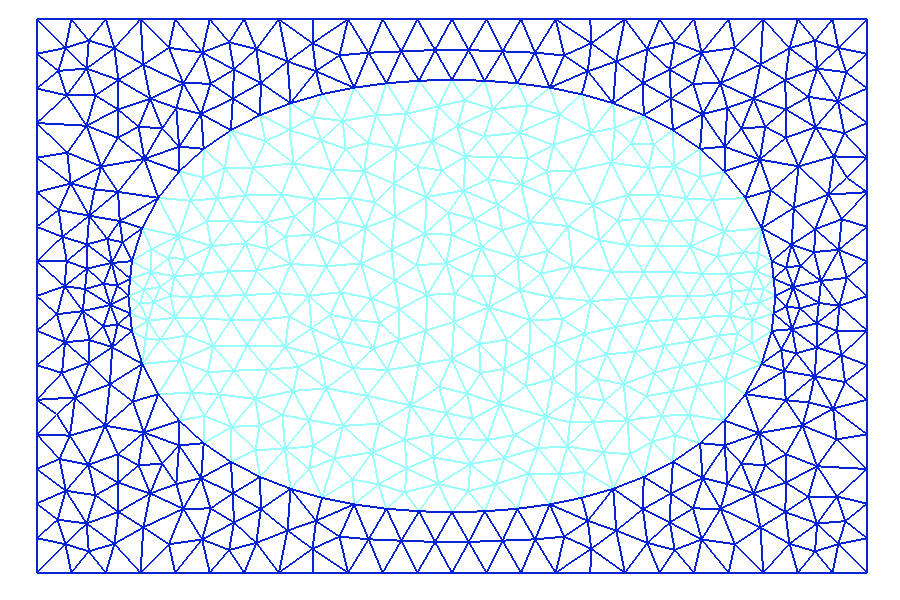
\includegraphics[width=.45\textwidth]{figures/remeshing_50.png}}\quad
 \subfloat[][]{
 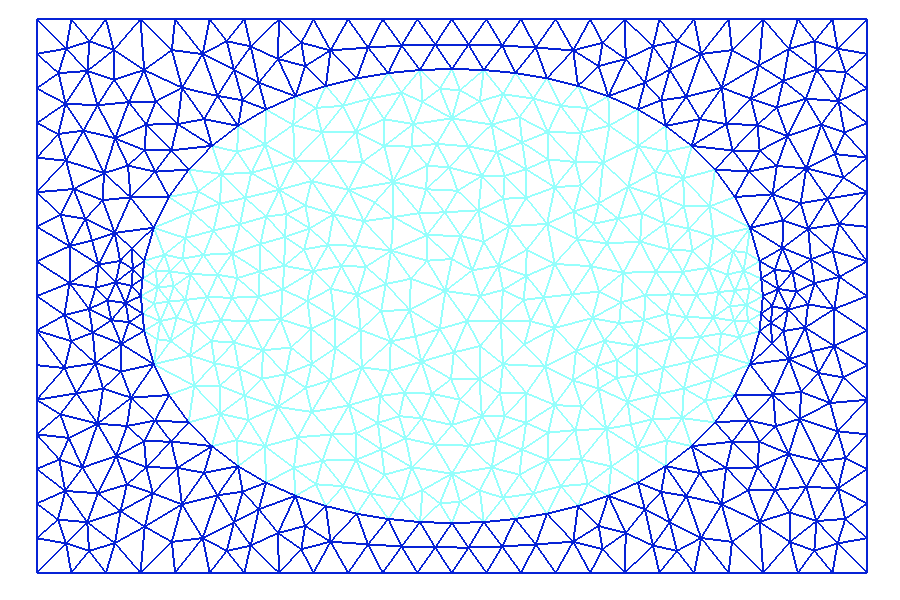
\includegraphics[width=.45\textwidth]{figures/remeshing_100.png}}\\
 \subfloat[][]{
 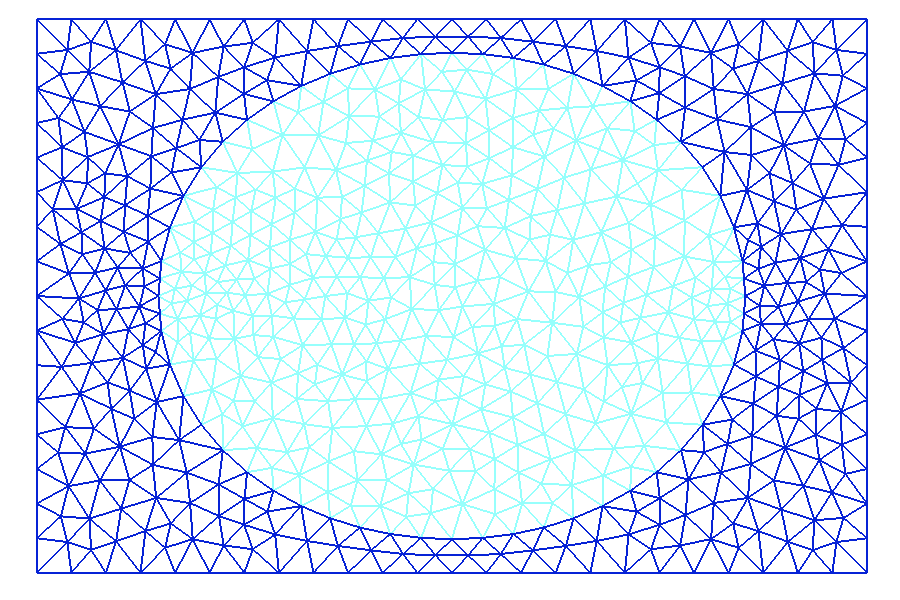
\includegraphics[width=.45\textwidth]{figures/remeshing_200.png}}\quad
 \subfloat[][]{
 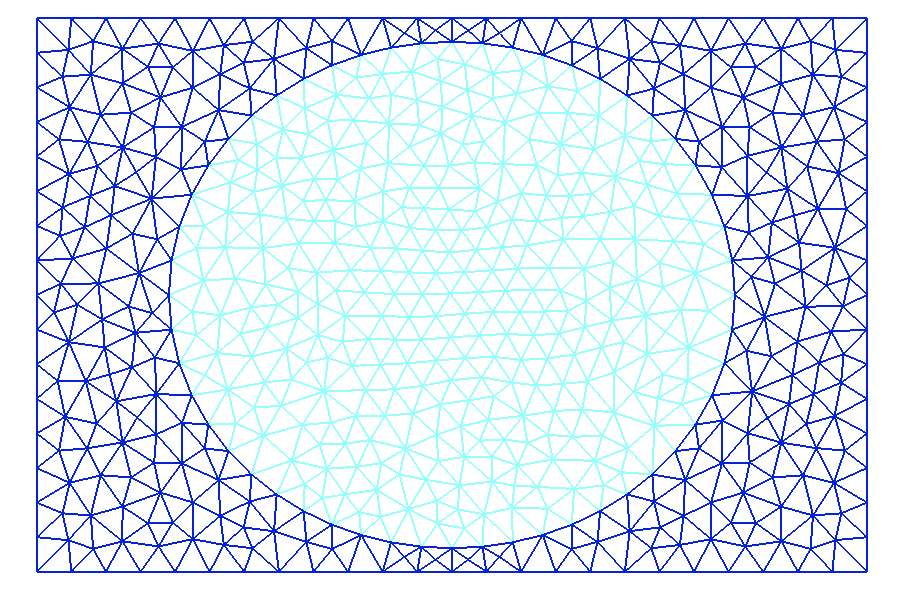
\includegraphics[width=.45\textwidth]{figures/remeshing_300.png}}
 \caption{Surface diffusion with an ellipse as initial condition coupled with
the bulk.}
 \label{fig:sd_ellipse_bulk}
\end{figure}

In Fig. \ref{fig:sd_ellipse_bulk} there are 4 snapshots of the simulation at
time $t=5$, $t=10$, $t=20$ and $t=30$, respectively. The edges of the rectangle
have length 6 and 4, respectively. The initial ellipse has semi-axes of length 5
and 3 along the x-axis and the y-axis, respectively. The number of mesh elements
for the interface is constant and equal to 52 elements. Obviously the number of
nodes is 52. The time step is constant and equal to $\tau=0.1$.
\newline

Since over the interface we are solving the same problem of Example
\ref{subsubsec:sd_ellipse} the evolution of the interface is the same.
Nevertheless, the sub-grid is coupled to the bulk now. Therefore when it
evolves, it moves also the nodes of the grid. For this reason the quality of the
mesh changes at each time-step.

The module performs a complete ``re-meshing'' of the bulk at certain time-steps
in order to improve the quality of the grid. Obviously the boundary of the bulk
and the interface are kept fixed during the re-mesh process.

\newpage

\section{Future work}

\subsection{Project plan}

Up to now, there are several things which I have to do in the following months.
Some of them should be quite straightforward while other will be more
challenging. A very rough plan is the following.
\newline

First of all I am going to extend the module \verb|dune-dynamic-grid| adding
some mesh quality controls and some algorithms to perform a mesh smoothing.

These two features are necessary because it is not feasible to rebuild the mesh
at each time step, since that is computationally very expensive compared to a
smoothing.
\newline

After that, the next step will be solution of the Navier--Stokes equation in
the bulk. This will result in a new module called \verb|dune-bulk|. The
simulator for the bulk problem will interact with the simulator for the
interface problem thanks to the module \verb|dune-coupled|.

So far, the module \verb|dune-coupled| manages only the geometrical coupling and
the simulator for the interface. For this reason I need also to work on this
module.
\newline

Finally, an optional feature which I would like to add is a full support for
parallel running for all the modules at least for 3-D problems. Actually some
part are already in parallel and some others are very simple to parallelize.
Nevertheless, this goal is quite difficult to achieve globally due to the
complex mesh management. I am confident that also a partial support to parallel
runs will boost up the code very much allowing faster computations.

\newpage

\section{Courses and conferences}

\subsection{Courses for academic credits}

This year I took the following courses:
\begin{itemize}
\item \gr{Manifolds}, Master Course, 30 hours;
\item \gr{Theory of PDE's}, TCC, 20 hours;
\item \gr{Advanced Finite Element Theory}, TCC, 20 hours;
\item \gr{Pseudo Differential Operators}, TCC, 20 hours;
\end{itemize}
completing 90 hours over the 100 hours which I have to do in my first two years
of Ph.D. .

\subsection{Courses for Graduate School}

In compliance with College regulations about Transferable Skills, I have already
attended four courses given by the Graduate School, precisely the following:

\begin{itemize}
\item \gr{Research Skills \& Development}, (RSD) Course, 3 courses;
\item \gr{Negotiation Skills for Researchers}, 1 course.
\end{itemize}

Moreover, I have completed the \gr{Plagiarism Awareness} course and I have met
College Postgraduate Research English requirement.

\subsection{Conferences}

I attended the conference Numerical Analysis for Partial Differential Equations,
held by University of Sussex, 18 - 20 June 2014.

\newpage
\bibliographystyle{siam} % plain
\bibliography{../../bib/robert_refs,../../bib/marco_refs}

\end{document}
